\documentclass[a4paper,12pt]{article}
\usepackage{xcolor}
\usepackage{algorithm}
\usepackage{algorithm}
\usepackage{algpseudocode}
\usepackage{amsmath,amsfonts,amssymb}
\usepackage{geometry}
\usepackage{fancyhdr}
\usepackage{graphicx}
\usepackage{subcaption}
\usepackage{caption}
\usepackage{titlesec}
\usepackage{tikz}
\usepackage{booktabs}
\usepackage{array}
\usetikzlibrary{positioning,arrows.meta} % Load the positioning library

\usetikzlibrary{shadows}
\usepackage{tcolorbox}
\usepackage{float}
\usepackage{lipsum}
\usepackage{mdframed}
\usepackage{pagecolor}
\usepackage{mathpazo}   % Palatino font (serif)
\usepackage{microtype}  % Better typography

% Page background color
\pagecolor{gray!10!white}

% Geometry settings
\geometry{margin=0.5in}
\pagestyle{fancy}
\fancyhf{}

% Fancy header and footer
\fancyhead[C]{\textbf{\color{blue!80}CS726 Programming Assignment -- 2 Report}}
\fancyhead[R]{\color{blue!80}Bayesian Bunch}
\fancyfoot[C]{\thepage}

% Custom Section Color and Format with Sans-serif font
\titleformat{\section}
{\sffamily\color{purple!90!black}\normalfont\Large\bfseries}
{\thesection}{1em}{}

% Custom subsection format
\titleformat{\subsection}
{\sffamily\color{cyan!80!black}\normalfont\large\bfseries}
{\thesubsection}{1em}{}

% Stylish Title with TikZ (Enhanced with gradient)
\newcommand{\cooltitle}[1]{%
  \begin{tikzpicture}
    \node[fill=blue!20,rounded corners=10pt,inner sep=12pt, drop shadow, top color=blue!50, bottom color=blue!30] (box)
    {\Huge \bfseries \color{black} #1};
  \end{tikzpicture}
}
\usepackage{float} % Add this package

\newenvironment{solution}[2][]{%
    \begin{mdframed}[linecolor=blue!70!black, linewidth=2pt, roundcorner=10pt, backgroundcolor=yellow!10!white, skipabove=12pt, skipbelow=12pt]%
        \textbf{\large #2}
        \par\noindent\rule{\textwidth}{0.4pt}
}{
    \end{mdframed}
}

% Document title
\title{\cooltitle{CS726 Programming Assignment -- 2 Report}}
\author{
\textbf{Saksham Rathi (22B1003)}\\
\textbf{Sharvanee Sonawane (22B0943)}\\
\textbf{Deeksha Dhiwakar (22B0988)}\\
\small Department of Computer Science, \\
Indian Institute of Technology Bombay \\}
\date{}

\begin{document}
\maketitle

\section*{Denoising Diffusion Probabilistic Models}

Here are the results of unconditional DDPMs on various datasets (with respect to the number of time steps). We had fixed all other parameters (the best settings observed):

\begin{itemize}
  \item lbeta=0.0001
  \item ubeta=0.02
  \item lr=0.0001 (so that training loss decreases across epochs)
  \item n\_samples=10000
  \item n\_dim=2 (for helix it is 3)
  \item batch\_size=128 (to avoid CUDA memory errors and produce optimal results)
  \item epochs=40
\end{itemize}

\clearpage
\subsection*{Moons}

\begin{figure}[H]
  \centering
  \begin{minipage}{0.3\textwidth}
      \centering
      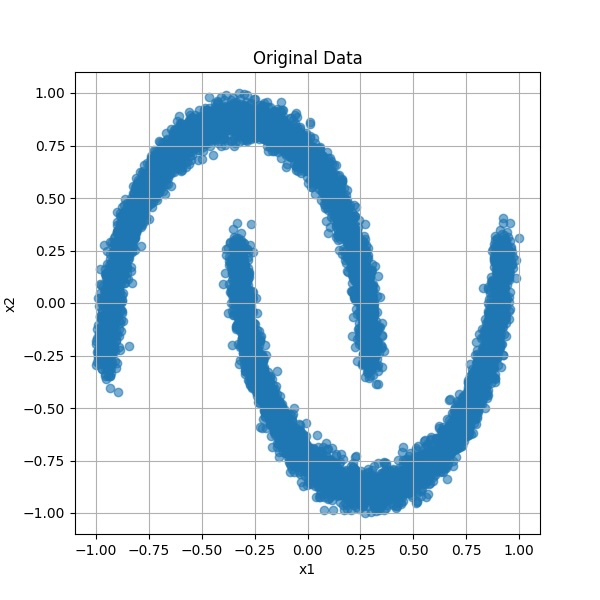
\includegraphics[width=\linewidth]{images/moon.jpg}
      \subcaption{Original Moons Dataset}
  \end{minipage}
  \begin{minipage}{0.3\textwidth}
      \centering
      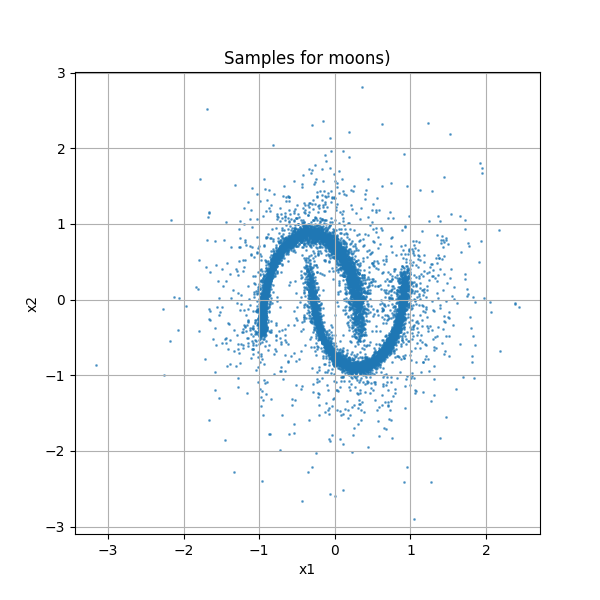
\includegraphics[width=\linewidth]{"images/Samples for ddpm_2_10_0.0001_0.02_moons.png"}
      \subcaption{Number of time steps = 10}
  \end{minipage}
  \begin{minipage}{0.3\textwidth}
      \centering
      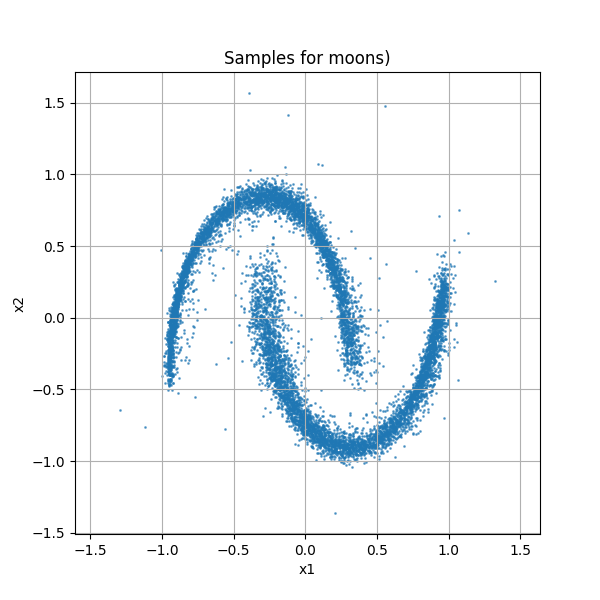
\includegraphics[width=\linewidth]{"images/Samples for ddpm_2_50_0.0001_0.02_moons.png"}
      \subcaption{Number of time steps = 50}
  \end{minipage}

  \vspace{0.5cm}

  \begin{minipage}{0.3\textwidth}
      \centering
      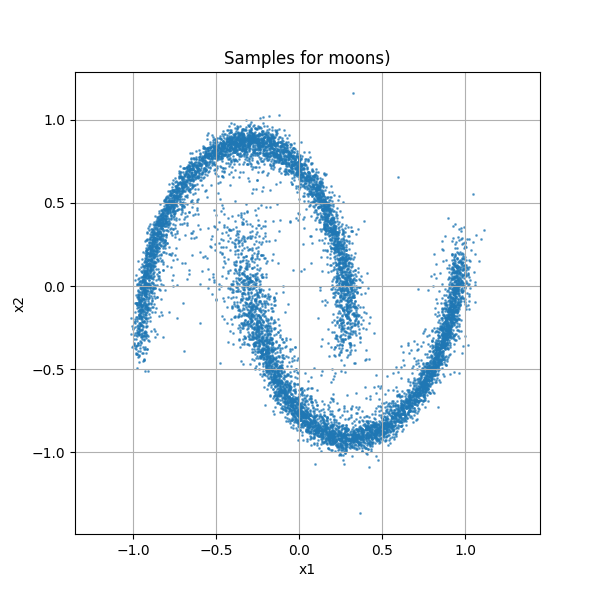
\includegraphics[width=\linewidth]{"images/Samples for ddpm_2_100_0.0001_0.02_moons.png"}
      \subcaption{Number of time steps = 100}
  \end{minipage}
  \begin{minipage}{0.3\textwidth}
      \centering
      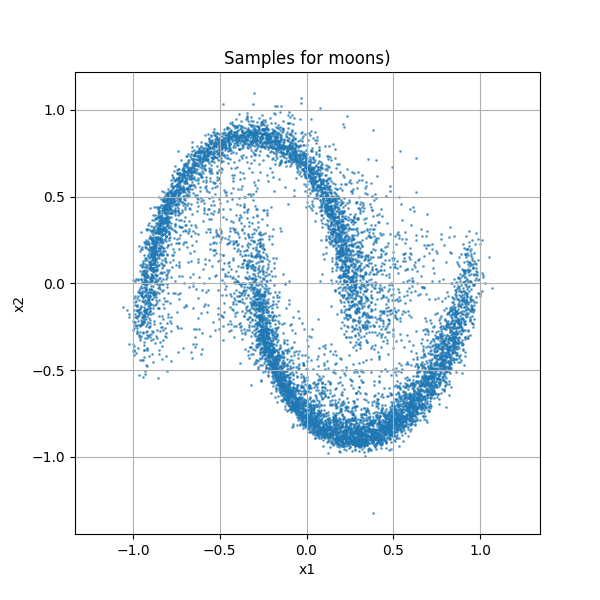
\includegraphics[width=\linewidth]{"images/Samples for ddpm_2_150_0.0001_0.02_moons.png"}
      \subcaption{Number of time steps = 150}
  \end{minipage}
  \begin{minipage}{0.3\textwidth}
      \centering
      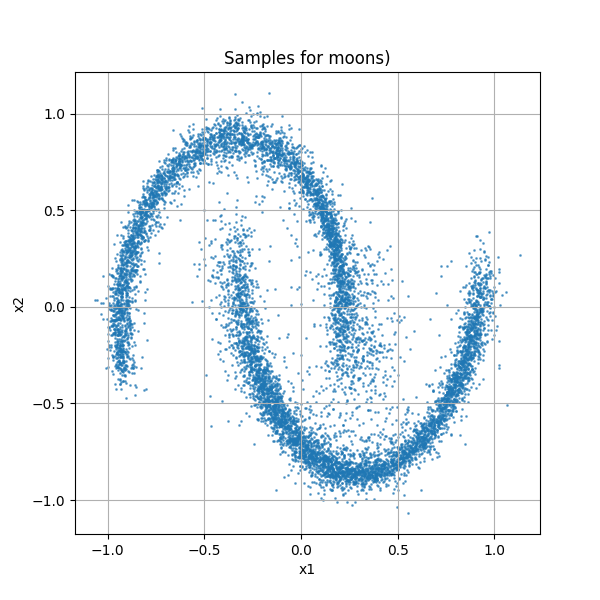
\includegraphics[width=\linewidth]{"images/Samples for ddpm_2_200_0.0001_0.02_moons.png"}
    \subcaption{Number of time steps = 200}
  \end{minipage}

  \caption{Moons Dataset}
\end{figure}

Here are the NLL values:
\begin{itemize}
  \item $T = 10$: 1.048
  \item $T = 50$: 0.9599
  \item $T = 100$: 0.9519
  \item $T = 150$: 0.9218
  \item $T = 200$: 0.9321
\end{itemize}

As, we can see from both NLL values and the images, $T = 150$ performed the best.

\clearpage



\subsection*{Blobs}

\begin{figure}[H]
  \centering
  \begin{minipage}{0.3\textwidth}
      \centering
      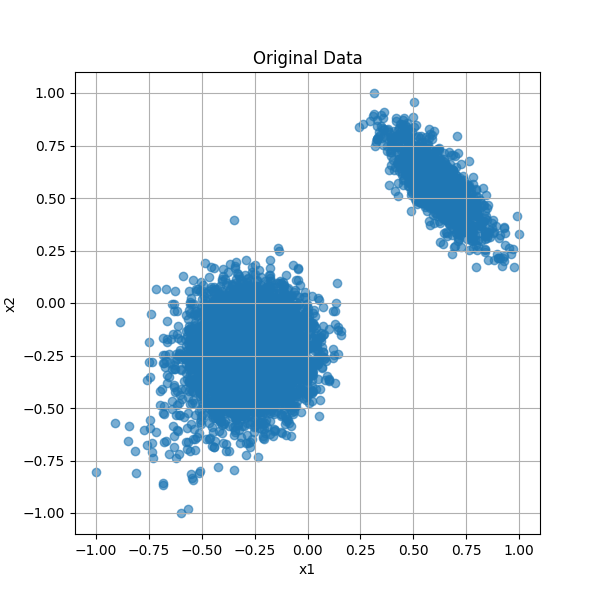
\includegraphics[width=\linewidth]{images/blobs.png}
      \subcaption{Original Blobs Dataset}
  \end{minipage}
  \begin{minipage}{0.3\textwidth}
      \centering
      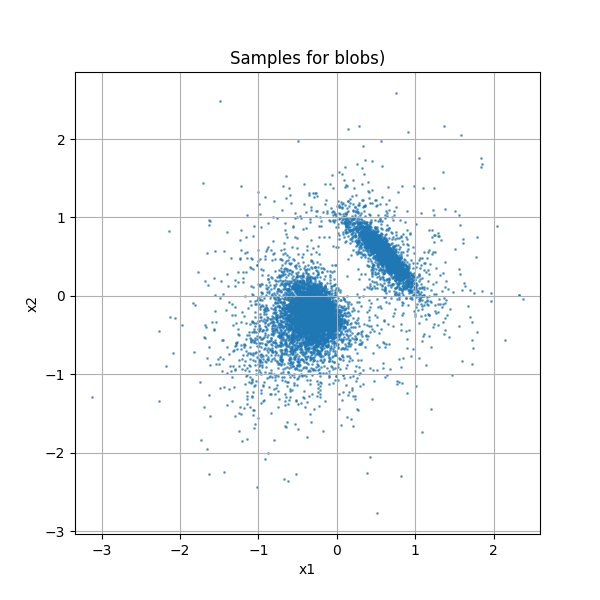
\includegraphics[width=\linewidth]{"images/Samples for ddpm_2_10_0.0001_0.02_blobs.png"}
      \subcaption{Number of time steps = 10}
  \end{minipage}
  \begin{minipage}{0.3\textwidth}
      \centering
      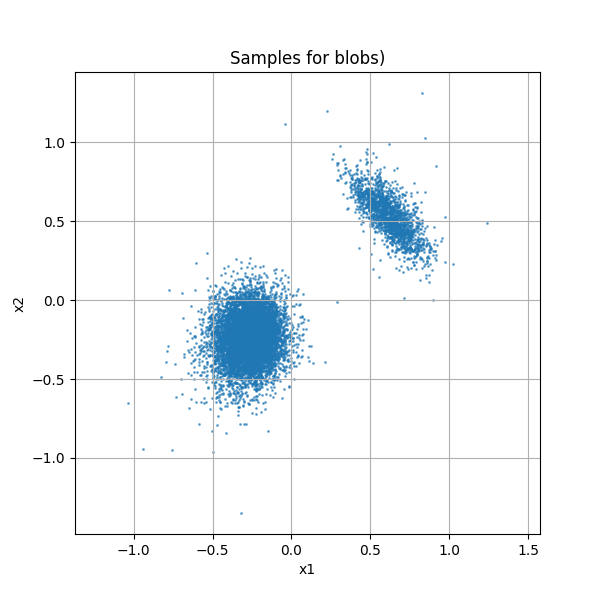
\includegraphics[width=\linewidth]{"images/Samples for ddpm_2_50_0.0001_0.02_blobs.png"}
      \subcaption{Number of time steps = 50}
  \end{minipage}

  \vspace{0.5cm}

  \begin{minipage}{0.3\textwidth}
      \centering
      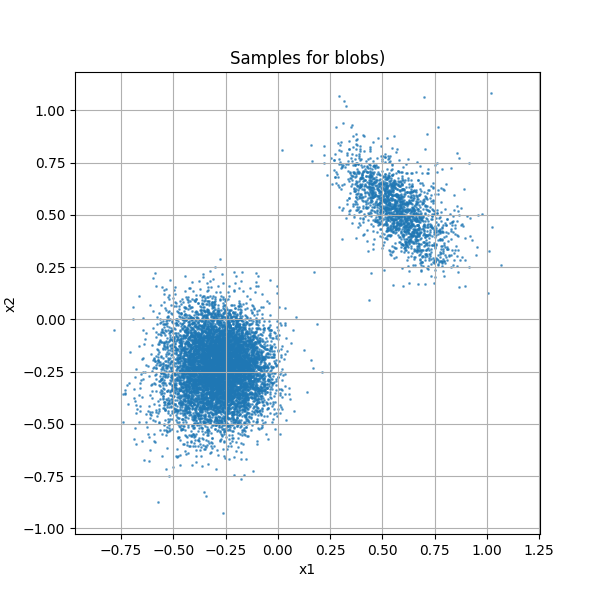
\includegraphics[width=\linewidth]{"images/Samples for ddpm_2_100_0.0001_0.02_blobs.png"}
      \subcaption{Number of time steps = 100}
  \end{minipage}
  \begin{minipage}{0.3\textwidth}
      \centering
      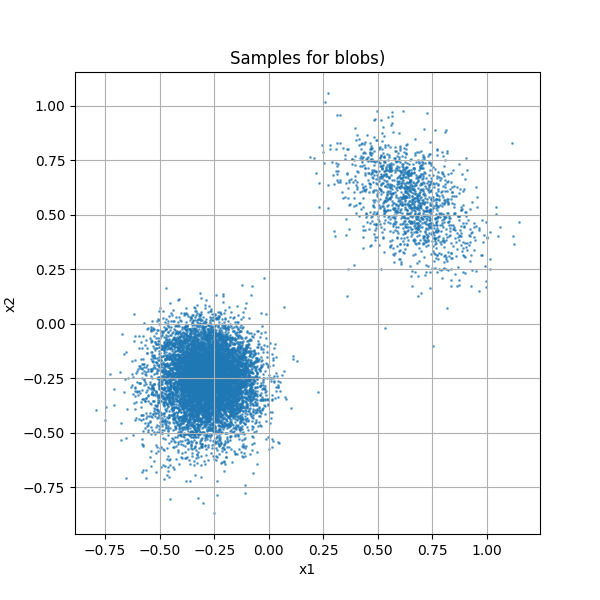
\includegraphics[width=\linewidth]{"images/Samples for ddpm_2_150_0.0001_0.02_blobs.png"}
      \subcaption{Number of time steps = 150}
  \end{minipage}
  \begin{minipage}{0.3\textwidth}
      \centering
      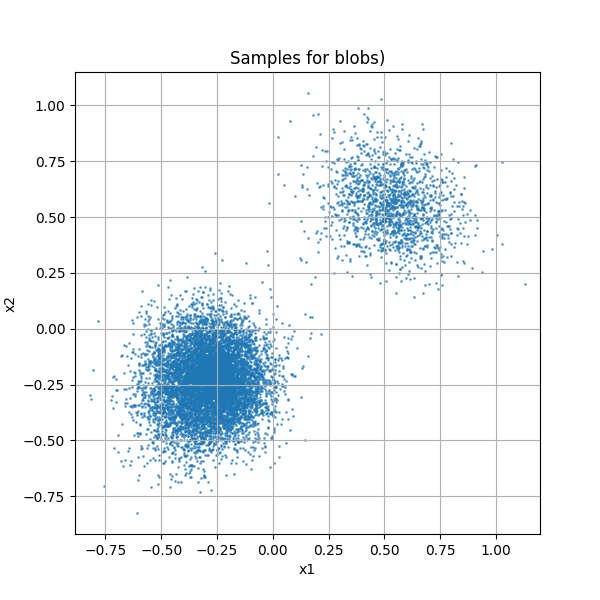
\includegraphics[width=\linewidth]{"images/Samples for ddpm_2_200_0.0001_0.02_blobs.png"}
    \subcaption{Number of time steps = 200}
  \end{minipage}

  \caption{Blobs Dataset}
\end{figure}

Here are the NLL values:
\begin{itemize}
  \item $T = 10$: 0.37
  \item $T = 50$: 0.0152
  \item $T = 100$: 0.0232
  \item $T = 150$: -0.0223
  \item $T = 200$: 0.0045
\end{itemize}

As, we can see from both NLL values and the images, $T = 150$ performed the best. Moreover, there is a sudden decrease in NLL from 10 to 50, which shows the significant impact of increasing the number of time steps.

\clearpage
\subsection*{Many-Circles}

\begin{figure}[H]
  \centering
  \begin{minipage}{0.3\textwidth}
      \centering
      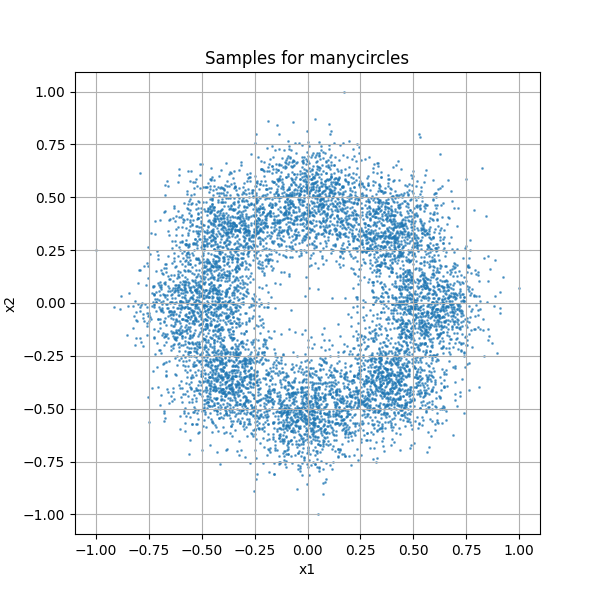
\includegraphics[width=\linewidth]{images/manycircles.png}
      \subcaption{Original ManyCircles Dataset}
  \end{minipage}
  \begin{minipage}{0.3\textwidth}
      \centering
      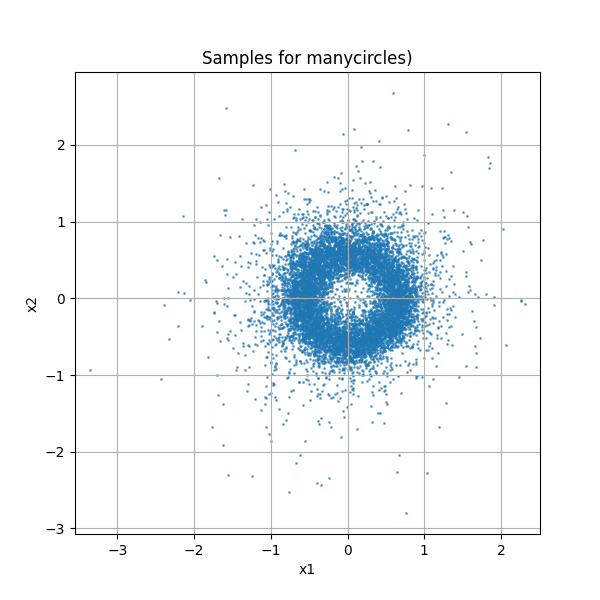
\includegraphics[width=\linewidth]{"images/Samples for ddpm_2_10_0.0001_0.02_manycircles.png"}
      \subcaption{Number of time steps = 10}
  \end{minipage}
  \begin{minipage}{0.3\textwidth}
      \centering
      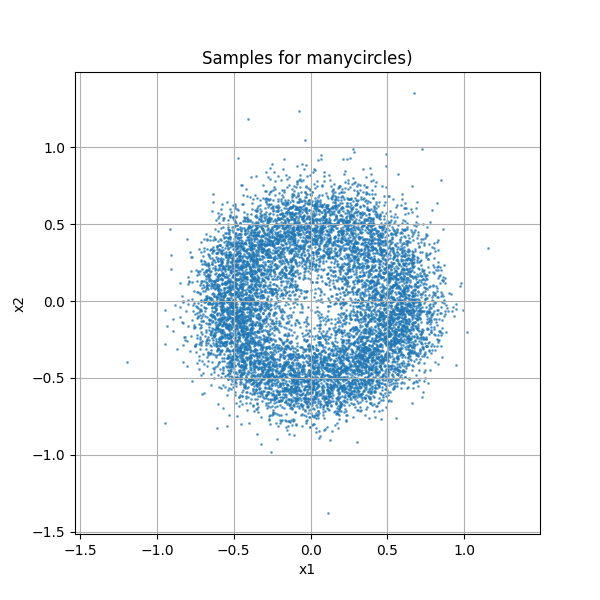
\includegraphics[width=\linewidth]{"images/Samples for ddpm_2_50_0.0001_0.02_manycircles.png"}
      \subcaption{Number of time steps = 50}
  \end{minipage}

  \vspace{0.5cm}

  \begin{minipage}{0.3\textwidth}
      \centering
      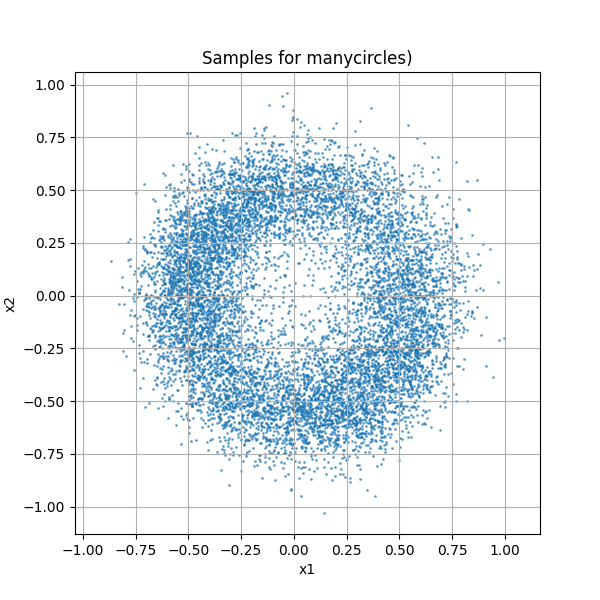
\includegraphics[width=\linewidth]{"images/Samples for ddpm_2_100_0.0001_0.02_manycircles.png"}
      \subcaption{Number of time steps = 100}
  \end{minipage}
  \begin{minipage}{0.3\textwidth}
      \centering
      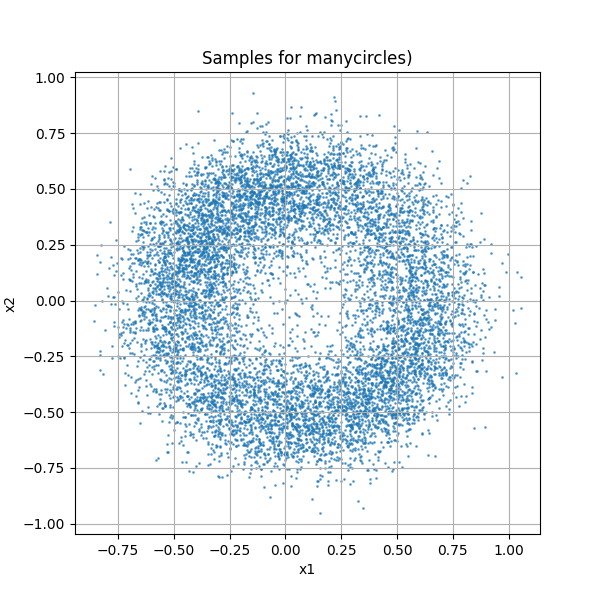
\includegraphics[width=\linewidth]{"images/Samples for ddpm_2_150_0.0001_0.02_manycircles.png"}
      \subcaption{Number of time steps = 150}
  \end{minipage}
  \begin{minipage}{0.3\textwidth}
      \centering
      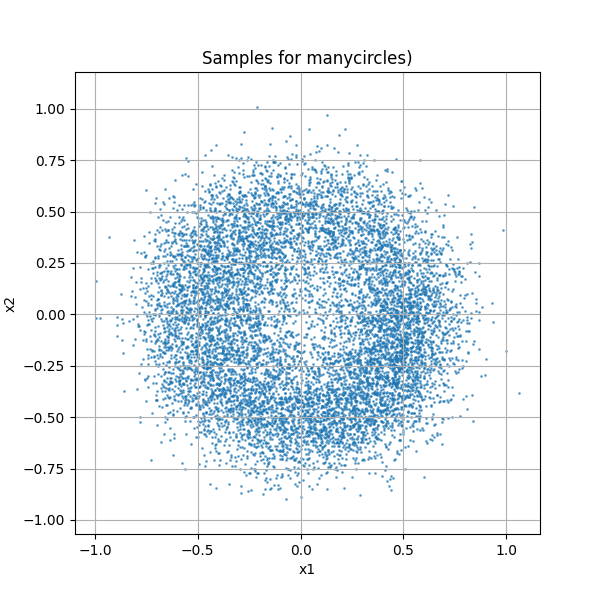
\includegraphics[width=\linewidth]{"images/Samples for ddpm_2_200_0.0001_0.02_manycircles.png"}
    \subcaption{Number of time steps = 200}
  \end{minipage}

  \caption{Many Circles Dataset}
\end{figure}

Here are the NLL values:
\begin{itemize}
  \item $T = 10$: 0.75
  \item $T = 50$: 0.548
  \item $T = 100$: 0.545
  \item $T = 150$: 0.558
  \item $T = 200$: 0.522
\end{itemize}

As, we can see from both NLL values and the images, $T = 200$ performed the best.

\clearpage

\subsection*{Circles}

\begin{figure}[H]
  \centering
  \begin{minipage}{0.3\textwidth}
      \centering
      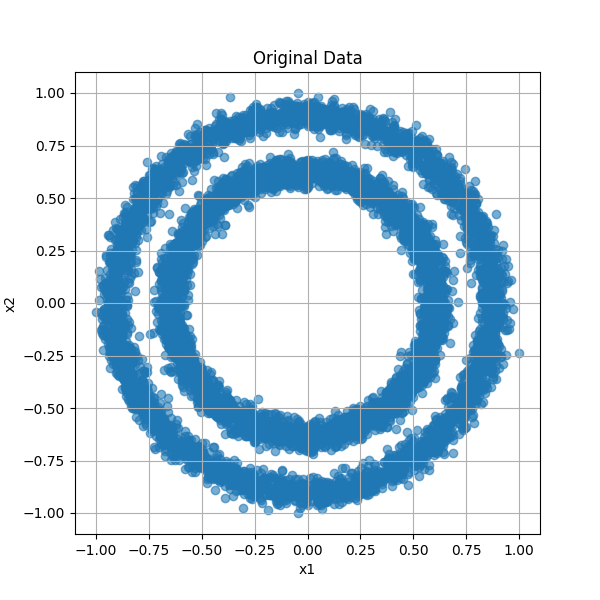
\includegraphics[width=\linewidth]{images/circles.png}
      \subcaption{Original Circles Dataset}
  \end{minipage}
  \begin{minipage}{0.3\textwidth}
      \centering
      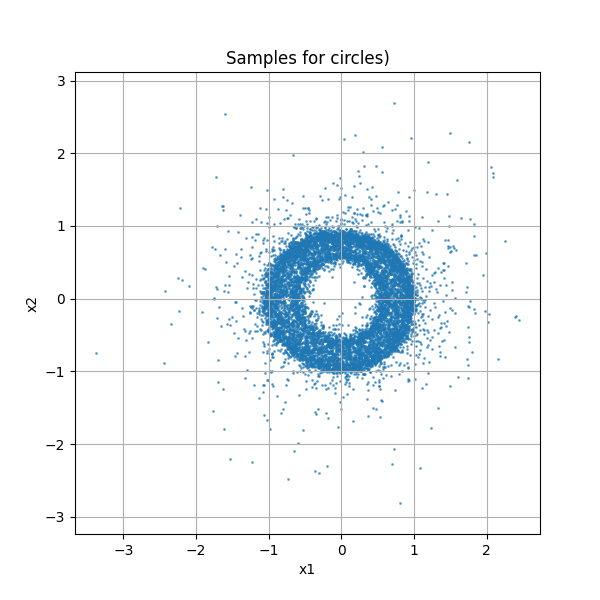
\includegraphics[width=\linewidth]{"images/Samples for ddpm_2_10_0.0001_0.02_circles.png"}
      \subcaption{Number of time steps = 10}
  \end{minipage}
  \begin{minipage}{0.3\textwidth}
      \centering
      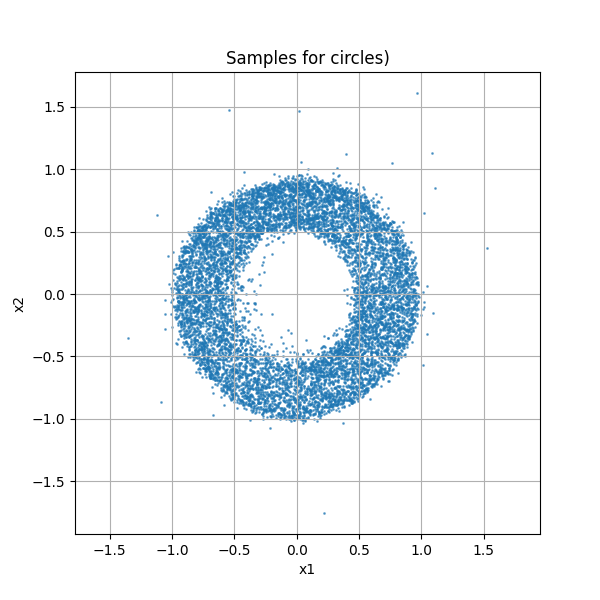
\includegraphics[width=\linewidth]{"images/Samples for ddpm_2_50_0.0001_0.02_circles.png"}
      \subcaption{Number of time steps = 50}
  \end{minipage}

  \vspace{0.5cm}

  \begin{minipage}{0.3\textwidth}
      \centering
      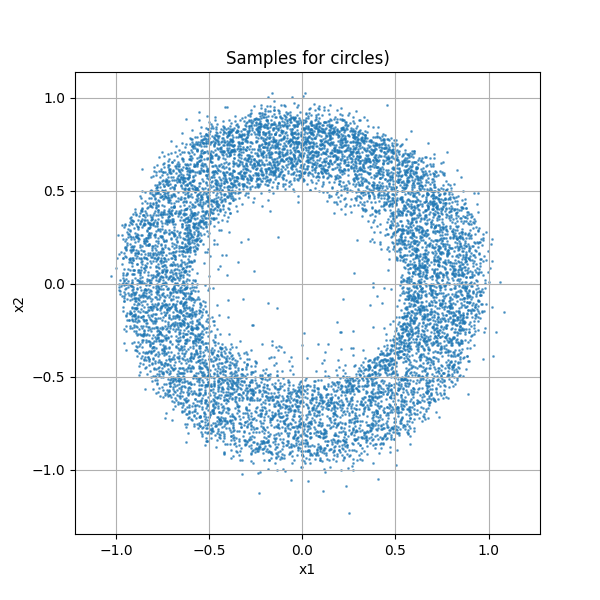
\includegraphics[width=\linewidth]{"images/Samples for ddpm_2_100_0.0001_0.02_circles.png"}
      \subcaption{Number of time steps = 100}
  \end{minipage}
  \begin{minipage}{0.3\textwidth}
      \centering
      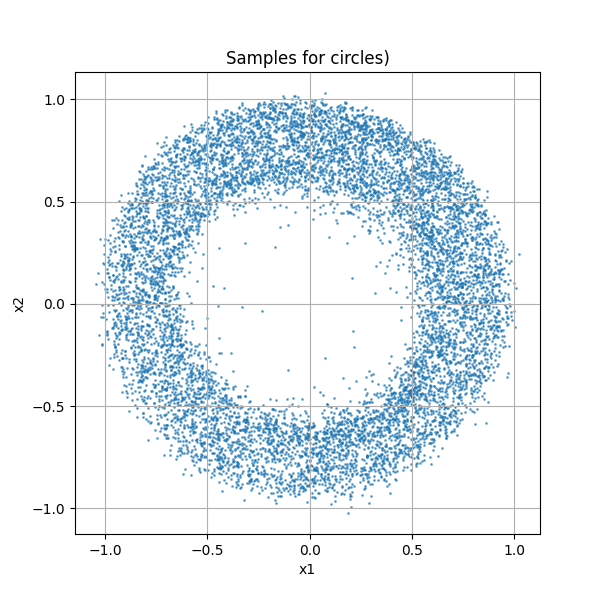
\includegraphics[width=\linewidth]{"images/Samples for ddpm_2_150_0.0001_0.02_circles.png"}
      \subcaption{Number of time steps = 150}
  \end{minipage}
  \begin{minipage}{0.3\textwidth}
      \centering
      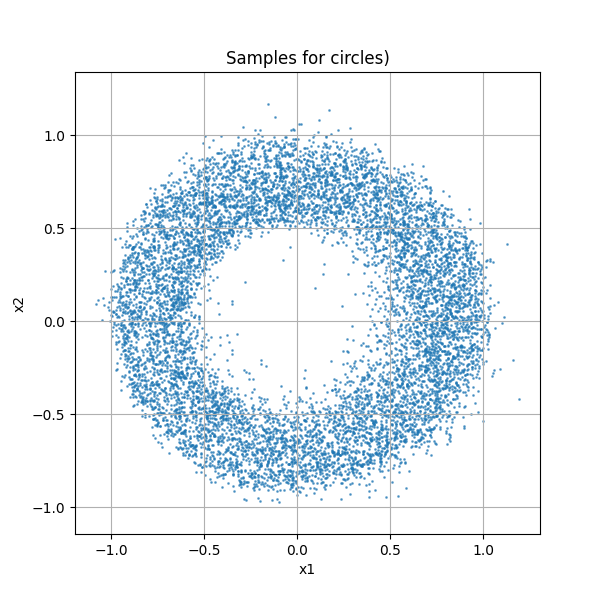
\includegraphics[width=\linewidth]{"images/Samples for ddpm_2_200_0.0001_0.02_circles.png"}
    \subcaption{Number of time steps = 200}
  \end{minipage}

  \caption{Circles Dataset}
\end{figure}


Here are the NLL values:
\begin{itemize}
  \item $T = 10$: 1.081
  \item $T = 50$: 0.991
  \item $T = 100$: 0.9869
  \item $T = 150$: 1.004
  \item $T = 200$: 0.992
\end{itemize}


\clearpage

\subsection*{Helix}

\begin{figure}[H]
  \centering
  \begin{minipage}{0.3\textwidth}
      \centering
      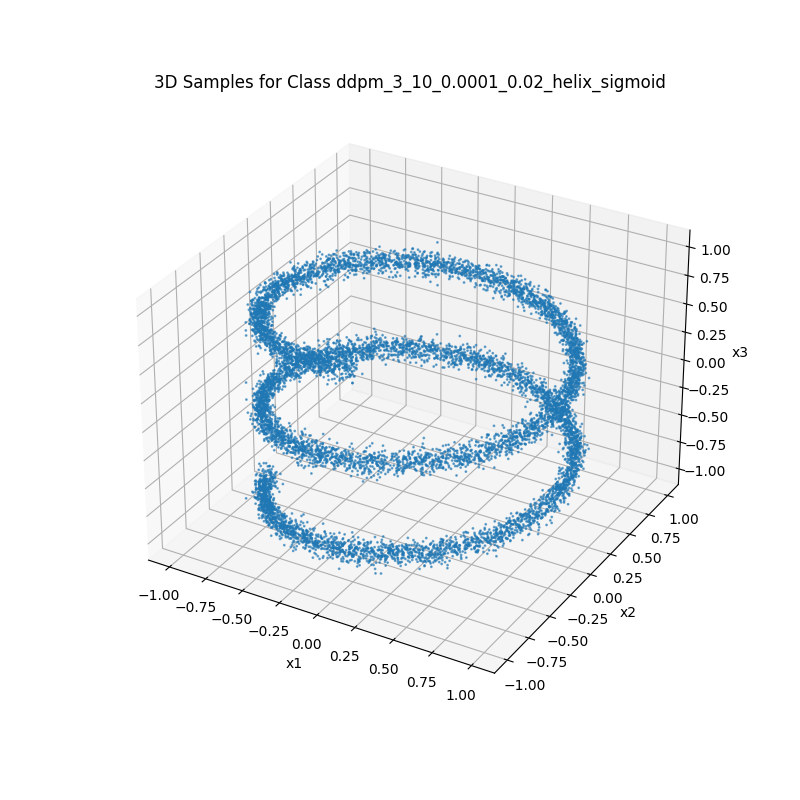
\includegraphics[width=\linewidth]{images/helix.png}
      \subcaption{Original Helix Dataset}
  \end{minipage}
  \begin{minipage}{0.3\textwidth}
      \centering
      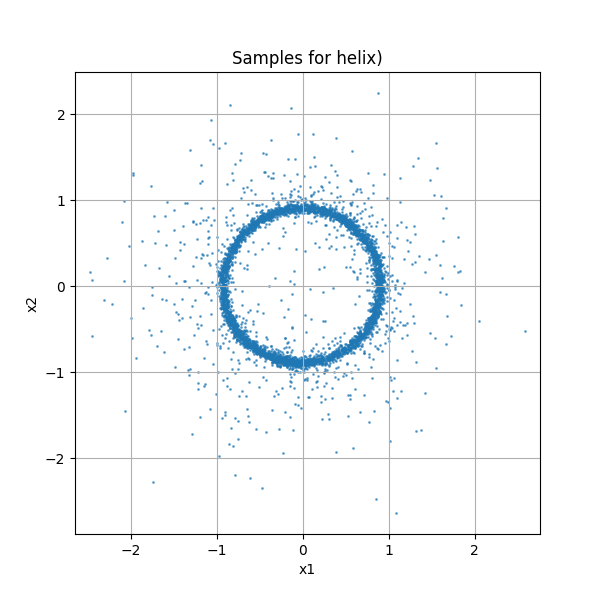
\includegraphics[width=\linewidth]{"images/Samples for ddpm_3_10_0.0001_0.02_helix_sigmoid.png"}
      \subcaption{Number of time steps = 10}
  \end{minipage}
  \begin{minipage}{0.3\textwidth}
      \centering
      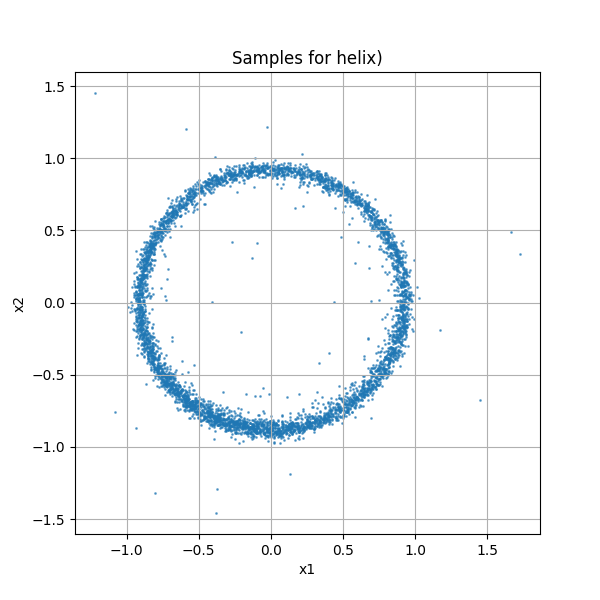
\includegraphics[width=\linewidth]{"images/Samples for ddpm_3_50_0.0001_0.02_helix_sigmoid.png"}
      \subcaption{Number of time steps = 50}
  \end{minipage}

  \vspace{0.5cm}

  \begin{minipage}{0.3\textwidth}
      \centering
      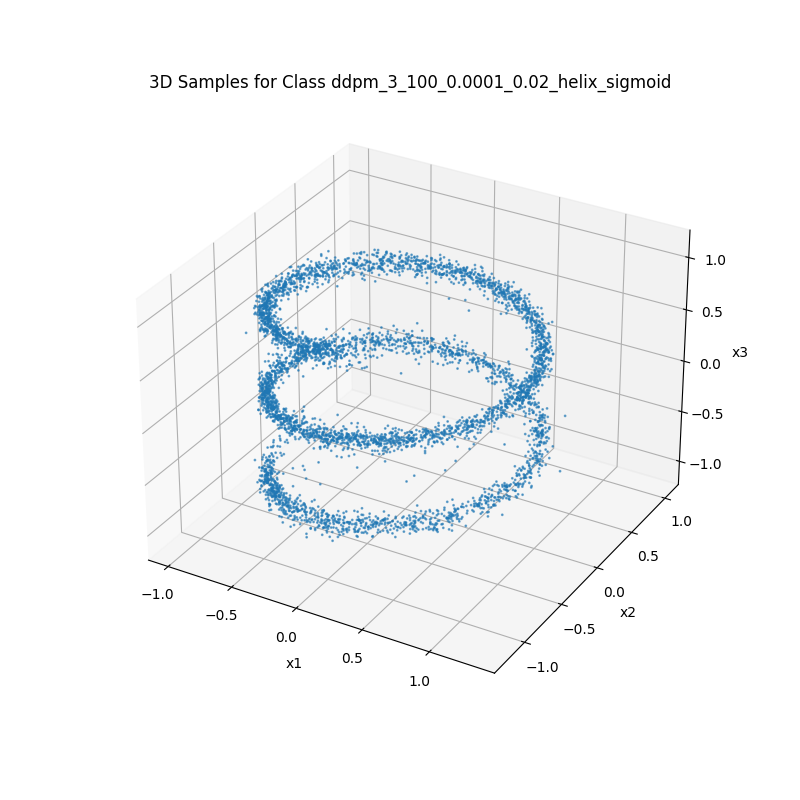
\includegraphics[width=\linewidth]{"images/Samples for ddpm_3_100_0.0001_0.02_helix_sigmoid.png"}
      \subcaption{Number of time steps = 100}
  \end{minipage}
  \begin{minipage}{0.3\textwidth}
      \centering
      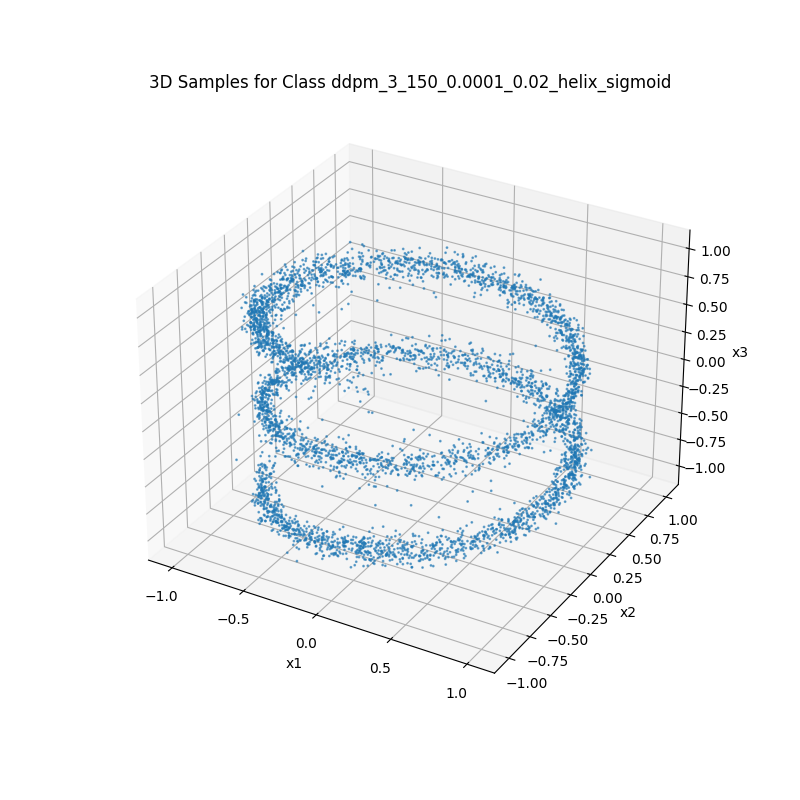
\includegraphics[width=\linewidth]{"images/Samples for ddpm_3_150_0.0001_0.02_helix_sigmoid.png"}
      \subcaption{Number of time steps = 150}
  \end{minipage}
  \begin{minipage}{0.3\textwidth}
      \centering
      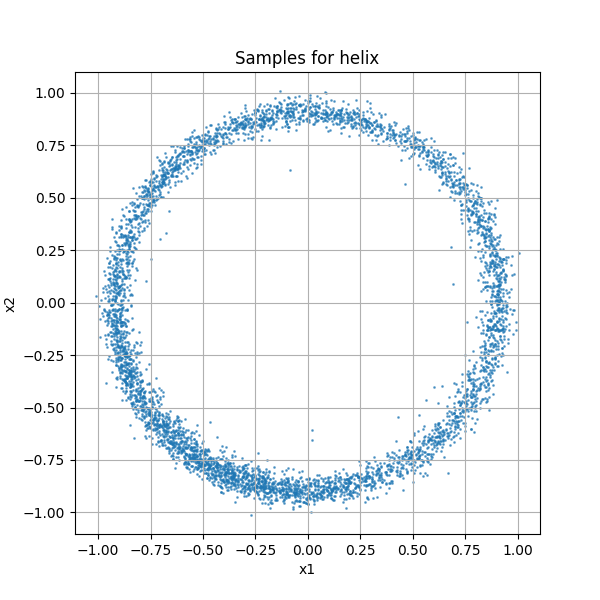
\includegraphics[width=\linewidth]{"images/Samples for ddpm_3_200_0.0001_0.02_helix_sigmoid.png"}
    \subcaption{Number of time steps = 200}
  \end{minipage}

  \caption{Helix Dataset}
\end{figure}


Here are the NLL values:
\begin{itemize}
  \item $T = 10$: 1.6179
  \item $T = 50$: 1.514
  \item $T = 100$: 1.5198
  \item $T = 150$: 1.528
  \item $T = 200$: 1.528
\end{itemize}

As we can see from the images (and the NLL values), 50 performs the best.

\subsection*{Noise Schedule Settings}
We trained the DDPM for various combinations of ubeta and lbeta values across all the datasets, and selected the best one using NLL value comparison. Here are the NLL values for the moons and blobs datasets:

\subsubsection*{Moons}

\begin{figure}[H]
  \centering
  \begin{minipage}{0.3\textwidth}
      \centering
      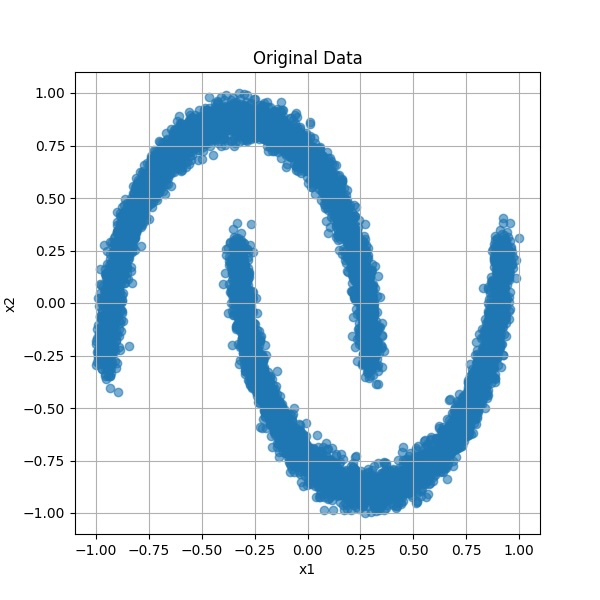
\includegraphics[width=\linewidth]{images/moon.jpg}
      \subcaption{Original Moons Dataset}
  \end{minipage}
  \begin{minipage}{0.3\textwidth}
      \centering
      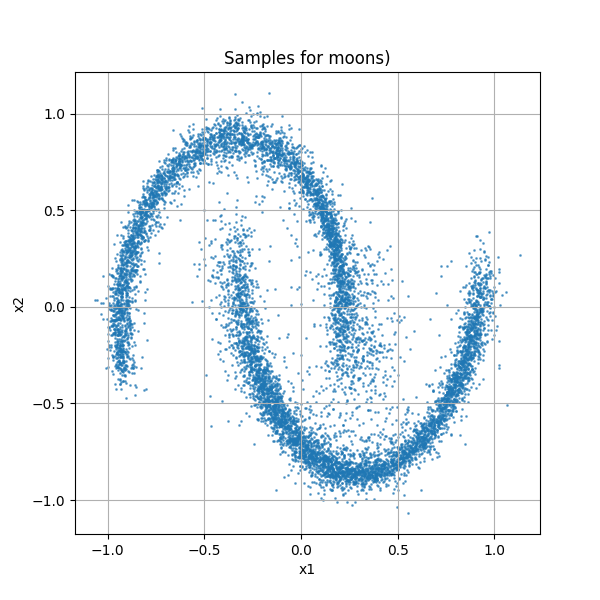
\includegraphics[width=\linewidth]{"images/Samples for ddpm_2_200_0.0001_0.02_moons_linear.png"}
      \subcaption{lbeta=0.0001, ubeta=0.02}
  \end{minipage}
  \begin{minipage}{0.3\textwidth}
      \centering
      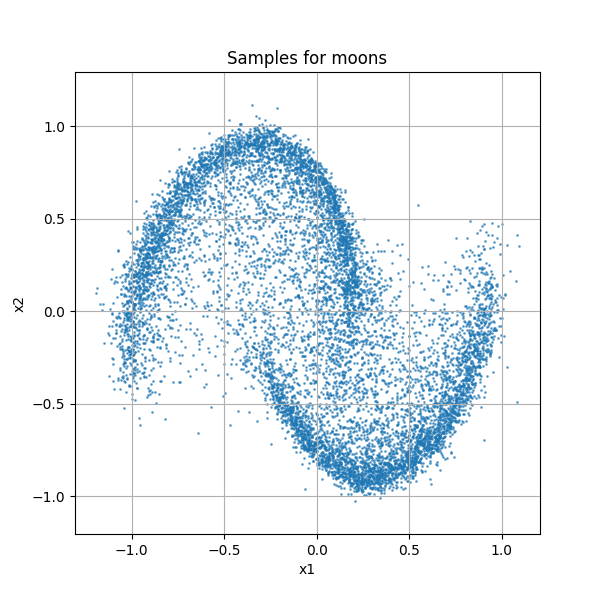
\includegraphics[width=\linewidth]{"images/Samples for ddpm_2_200_0.0001_0.05_moons_linear.png"}
      \subcaption{lbeta=0.0001, ubeta=0.05}
  \end{minipage}

  \vspace{0.5cm}

  \begin{minipage}{0.3\textwidth}
      \centering
      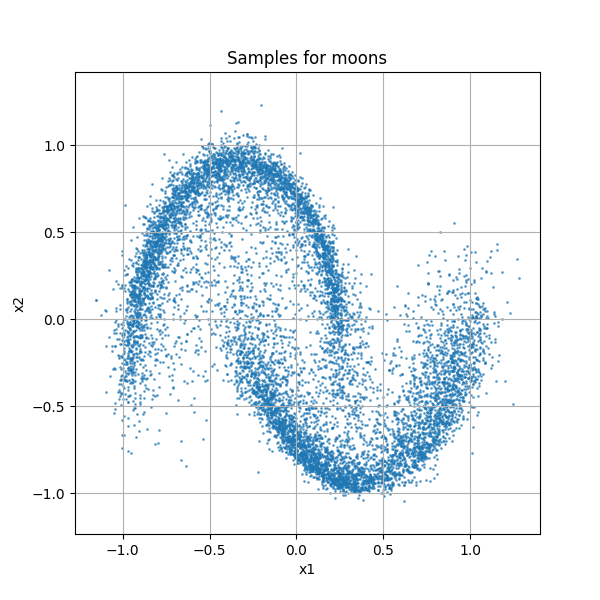
\includegraphics[width=\linewidth]{"images/Samples for ddpm_2_200_0.001_0.05_moons_linear.png"}
      \subcaption{lbeta=0.0005, ubeta=0.02}
  \end{minipage}
  \begin{minipage}{0.3\textwidth}
      \centering
      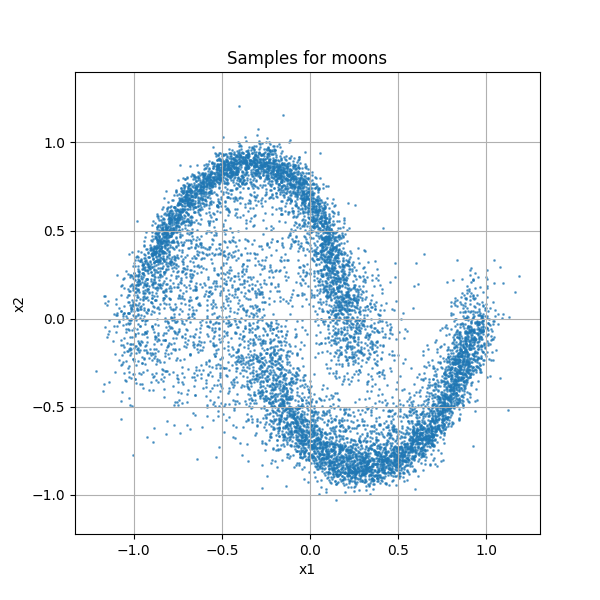
\includegraphics[width=\linewidth]{"images/Samples for ddpm_2_200_0.0005_0.05_moons_linear.png"}
      \subcaption{lbeta=0.0005, ubeta=0.05}
  \end{minipage}
  \begin{minipage}{0.3\textwidth}
      \centering
      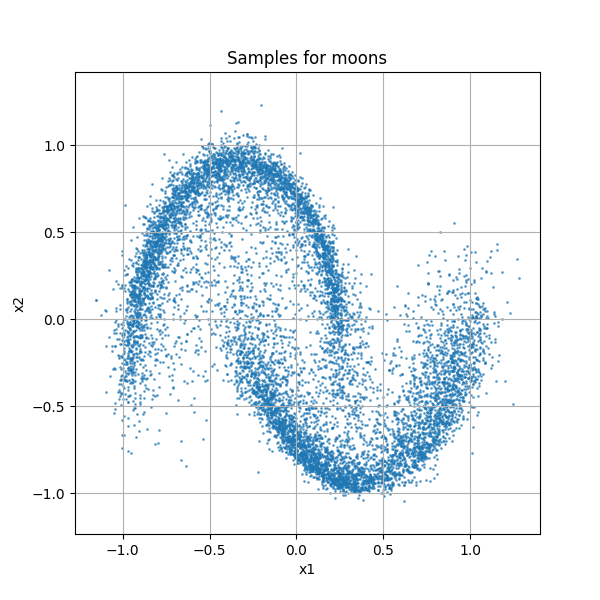
\includegraphics[width=\linewidth]{"images/Samples for ddpm_2_200_0.001_0.05_moons_linear.png"}
      \subcaption{lbeta=0.001, ubeta=0.05}
  \end{minipage}

  \caption{Moons Dataset}
\end{figure}

\begin{itemize}
  \item lbeta = 0.0001, ubeta = 0.02: 0.9184
  \item lbeta = 0.0001, ubeta = 0.05: 0.9223
  \item lbeta = 0.0005, ubeta = 0.02: 0.9321
  \item lbeta = 0.0005, ubeta = 0.05: 0.9265
  \item lbeta = 0.001, ubeta = 0.05: 0.9498
\end{itemize}

\subsubsection*{Blobs}

\begin{figure}[H]
  \centering
  \begin{minipage}{0.3\textwidth}
      \centering
      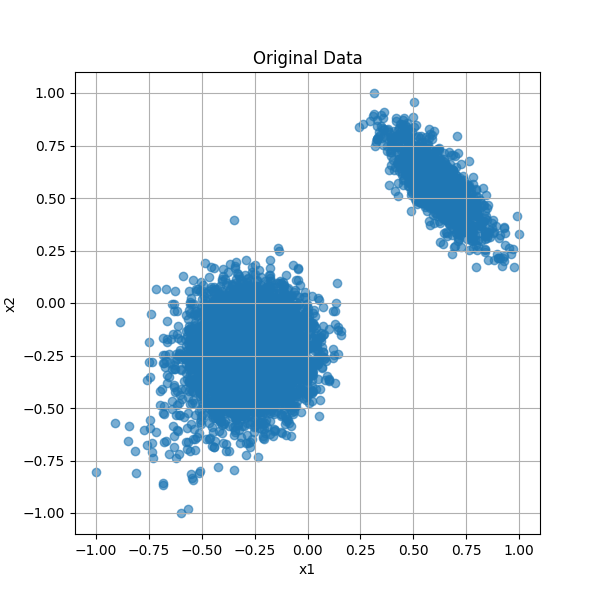
\includegraphics[width=\linewidth]{images/blobs.png}
      \subcaption{Original Blobs Dataset}
  \end{minipage}
  \begin{minipage}{0.3\textwidth}
      \centering
      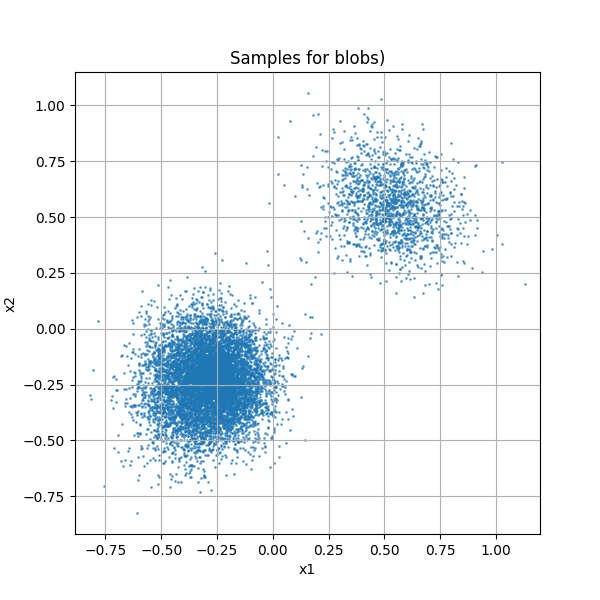
\includegraphics[width=\linewidth]{"images/Samples for ddpm_2_200_0.0001_0.02_blobs_linear.png"}
      \subcaption{lbeta=0.0001, ubeta=0.02}
  \end{minipage}
  \begin{minipage}{0.3\textwidth}
      \centering
      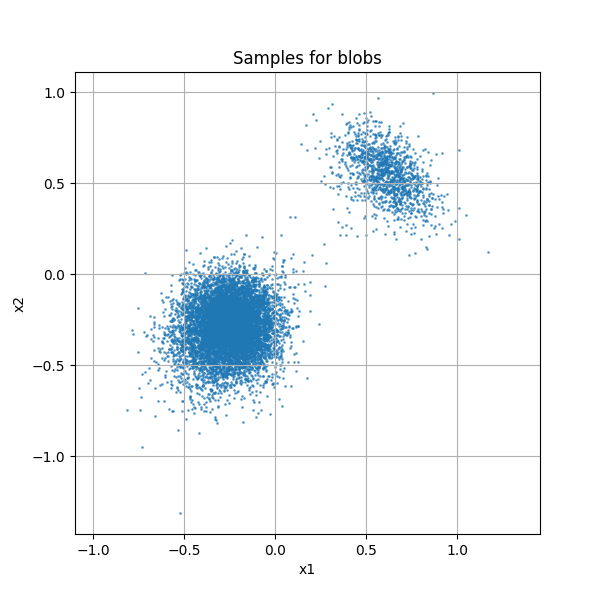
\includegraphics[width=\linewidth]{"images/Samples for ddpm_2_200_0.0001_0.05_blobs_linear.png"}
      \subcaption{lbeta=0.0001, ubeta=0.05}
  \end{minipage}

  \vspace{0.5cm}

  \begin{minipage}{0.3\textwidth}
      \centering
      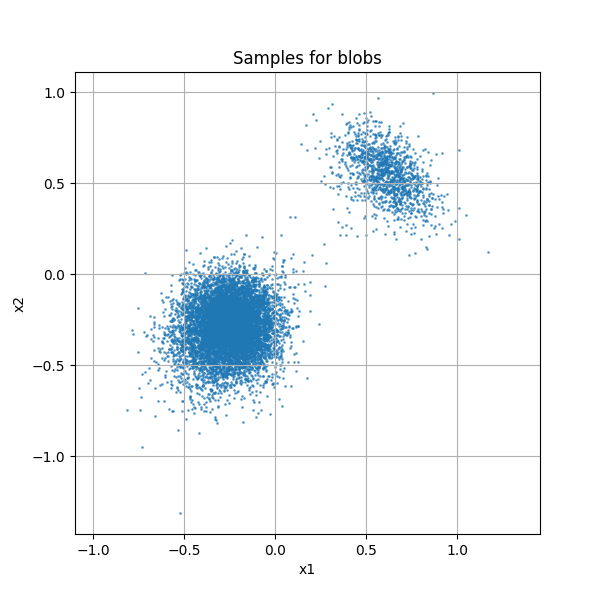
\includegraphics[width=\linewidth]{"images/Samples for ddpm_2_200_0.0005_0.02_blobs_linear.png"}
      \subcaption{lbeta=0.0005, ubeta=0.02}
  \end{minipage}
  \begin{minipage}{0.3\textwidth}
      \centering
      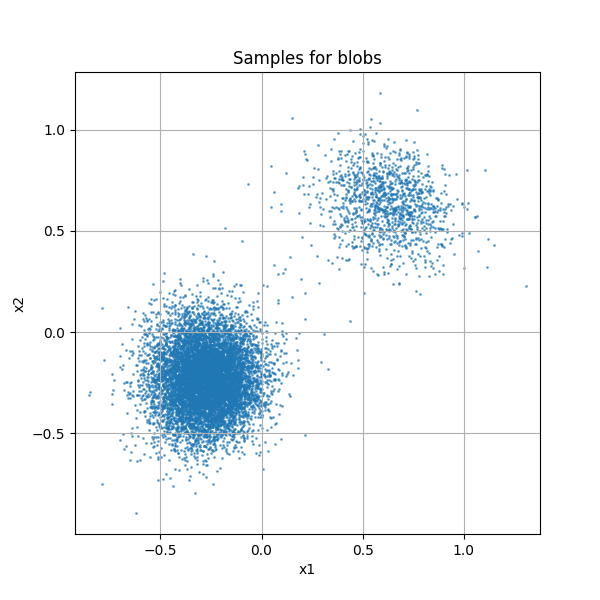
\includegraphics[width=\linewidth]{"images/Samples for ddpm_2_200_0.0005_0.05_blobs_linear.png"}
      \subcaption{lbeta=0.0005, ubeta=0.05}
  \end{minipage}
  \begin{minipage}{0.3\textwidth}
      \centering
      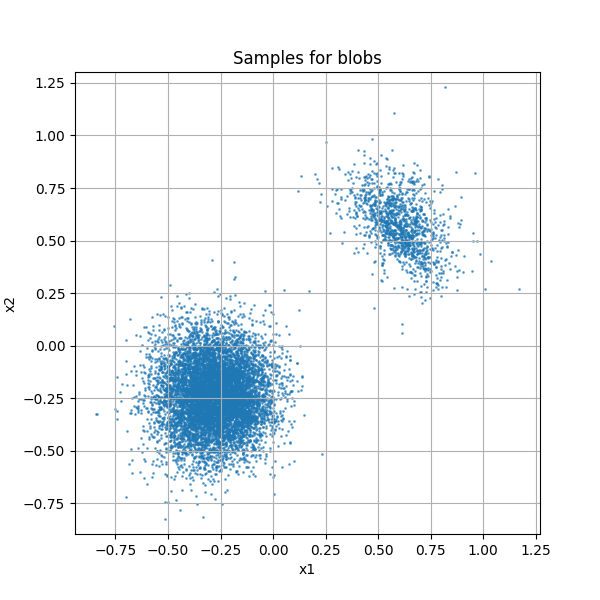
\includegraphics[width=\linewidth]{"images/Samples for ddpm_2_200_0.001_0.05_blobs_linear.png"}
      \subcaption{lbeta=0.001, ubeta=0.05}
  \end{minipage}

  \caption{Blobs Dataset}
\end{figure}

\begin{itemize}
  \item lbeta = 0.0001, ubeta = 0.02: -0.0145
  \item lbeta = 0.0001, ubeta = 0.05: -0.0102
  \item lbeta = 0.0005, ubeta = 0.02: -0.0099
  \item lbeta = 0.0005, ubeta = 0.05: -0.0104
  \item lbeta = 0.001, ubeta = 0.05: -0.0098
\end{itemize}
We observe similar NLL trends for the other datasets as well, leading us to conclude that lbeta=0.0001 and ubeta=0.02 are the best hyperparameters for the linear noise schedule.

\subsection*{Comparison with Cosine and Sigmoid Noise Schedules}
Along with the linear noise schedule, we have studied the effect of cosine and sigmoid noise schedules for the DDP model. The results of the comparison are as shown below. In each of the cases we have set the other hyperparameters as follows:
\begin{itemize}
  \item Number of time steps = 200
  \item lbeta=0.0001
  \item ubeta=0.02
  \item lr=0.0001
  \item n\_samples=10000
  \item n\_dim=2
  \item batch\_size=128
  \item epochs=40
\end{itemize}

\subsubsection*{Moons}
\begin{figure}[H]
  \centering
  \begin{minipage}{0.3\textwidth}
      \centering
      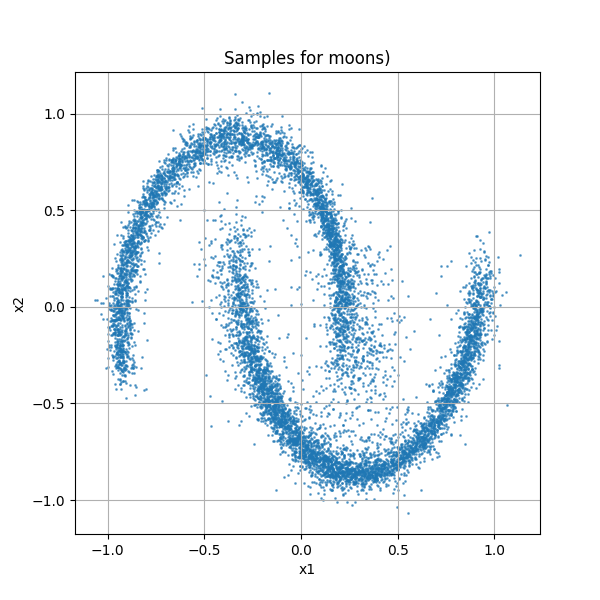
\includegraphics[width=\linewidth]{images/Samples for ddpm_2_200_0.0001_0.02_moons_linear.png}
      \subcaption{Linear Noise Schedule\\NLL=0.932}
  \end{minipage}
  \begin{minipage}{0.3\textwidth}
      \centering
      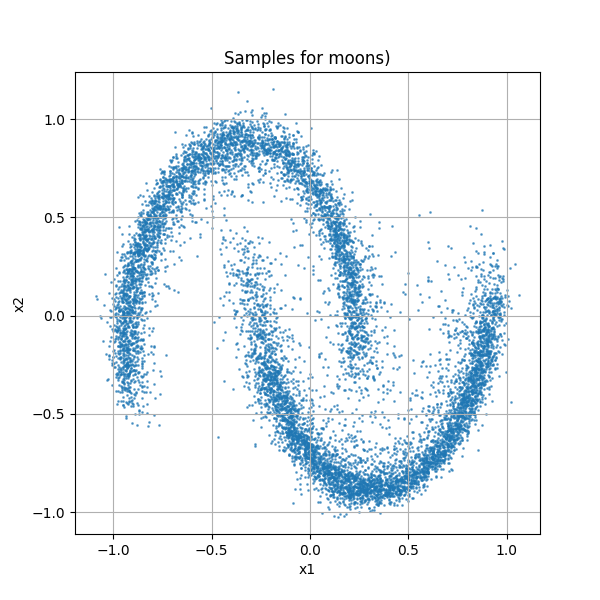
\includegraphics[width=\linewidth]{images/Samples for ddpm_2_200_0.0001_0.02_moons_cosine.png}
      \subcaption{Cosine Noise Schedule\\NLL=0.949}
  \end{minipage}
  \begin{minipage}{0.3\textwidth}
      \centering
      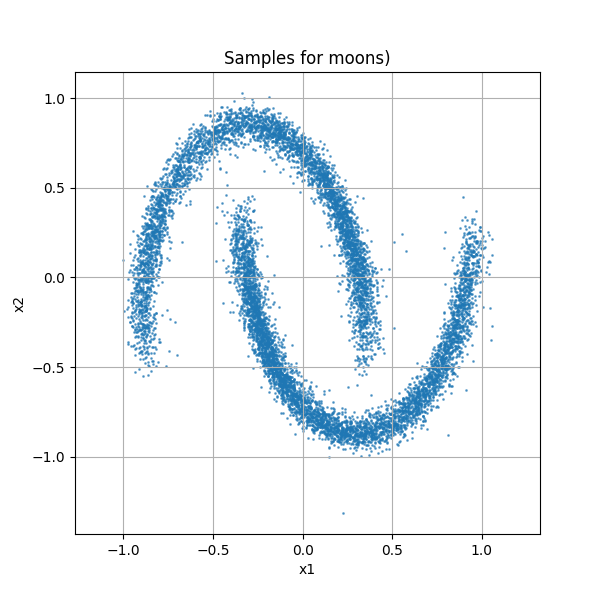
\includegraphics[width=\linewidth]{images/Samples for ddpm_2_200_0.0001_0.02_moons_sigmoid.png}
      \subcaption{Sigmoid Noise Schedule\\NLL=0.928}
  \end{minipage}
\end{figure}
In this case, we observe that the sigmoid noise schedule is the best out of the three.
\subsubsection*{Blobs}
\begin{figure}[H]
  \centering
  \begin{minipage}{0.3\textwidth}
      \centering
      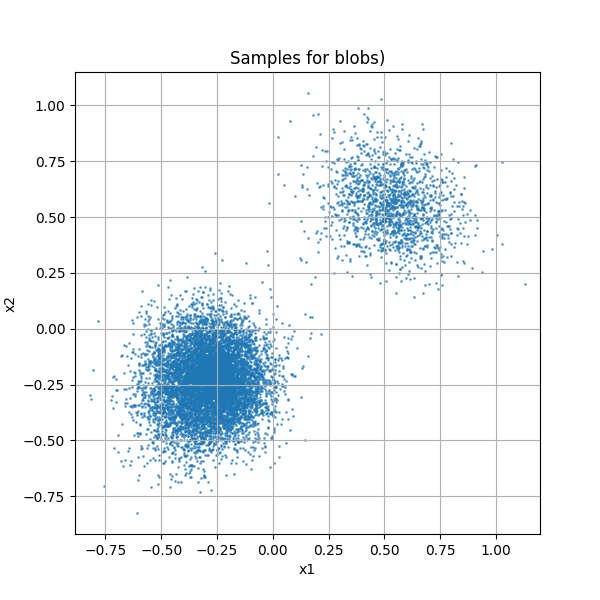
\includegraphics[width=\linewidth]{images/Samples for ddpm_2_200_0.0001_0.02_blobs_linear.png}
      \subcaption{Linear Noise Schedule\\NLL=0.0045}
  \end{minipage}
  \begin{minipage}{0.3\textwidth}
      \centering
      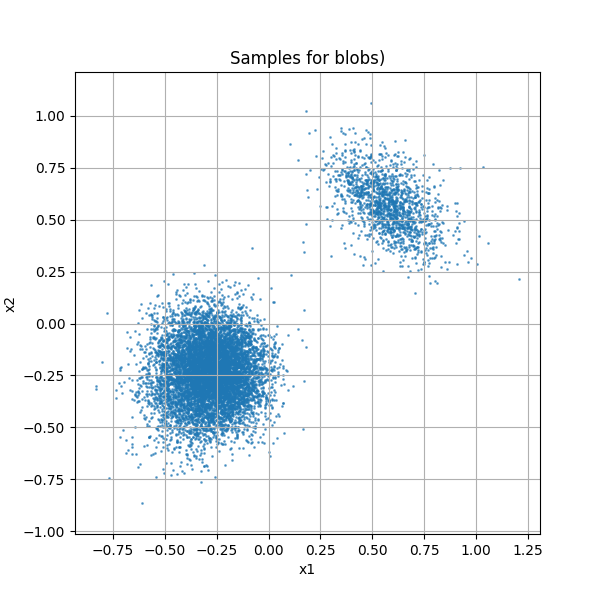
\includegraphics[width=\linewidth]{images/Samples for ddpm_2_200_0.0001_0.02_blobs_cosine.png}
      \subcaption{Cosine Noise Schedule\\NLL=0.0043}
  \end{minipage}
  \begin{minipage}{0.3\textwidth}
      \centering
      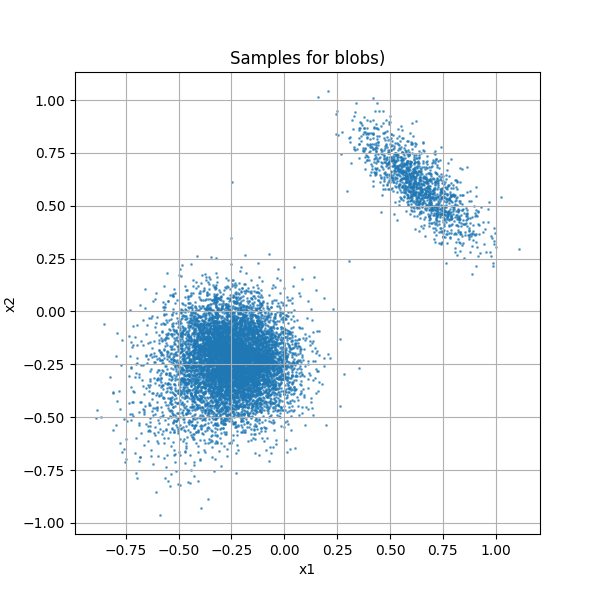
\includegraphics[width=\linewidth]{images/Samples for ddpm_2_200_0.0001_0.02_blobs_sigmoid.png}
      \subcaption{Sigmoid Noise Schedule\\NLL=0.0066}
  \end{minipage}
\end{figure}
In this case, we observe that the cosine noise schedule is the best out of the three.



\clearpage


\section*{Classifier-Free Guidance}

\subsection*{Difference between Guided Sampling and Conditional Sampling}
In conditional sampling, we model $p(x|y)$ directly, where $y$ is a conditioning variable (like a class label). During generation, we sample from this conditional distribution to get samples that match the condition.

In guided sampling (specifically classifier-free guidance), we train two models: one conditional $p(x|y)$ and one unconditional $p(x)$. During sampling, we interpolate between them with a guidance scale w:
\[\epsilon_\theta(x_t, t, y) = (1+w) * \epsilon_\theta(x_t, t, y) - w * \epsilon_\theta(x_t, t)\]
Firstly, guided sampling is more expensive in terms of computation required to train and sample points (almost double, since we are training two models, and using both of them to sample points). However, this guidance increases the impact of the conditioning information and can produce higher quality samples that better match the condition, but with a potential loss of diversity.

\subsection*{Effect of guidance scale}
We sampled points using CFG on a variety of guidance scale values, here are the images from the moon dataset:

\begin{figure}[H]
  \centering
  \begin{minipage}{0.3\textwidth}
      \centering
      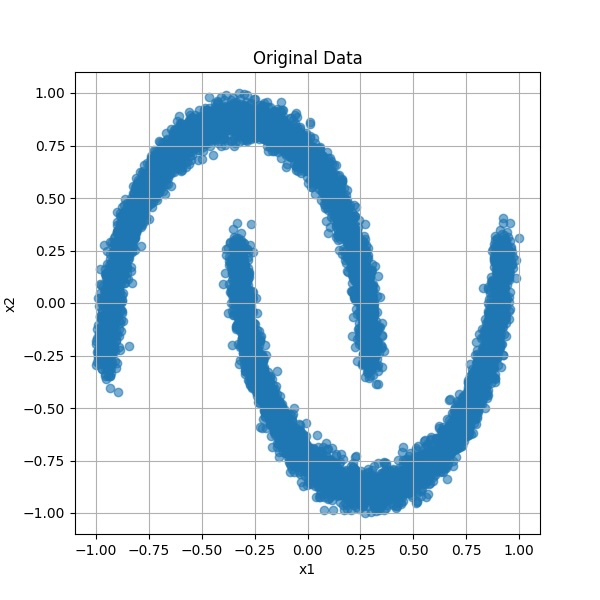
\includegraphics[width=\linewidth]{images/moon.jpg}
      \subcaption{Original Moons Dataset}
  \end{minipage}
  \begin{minipage}{0.3\textwidth}
      \centering
      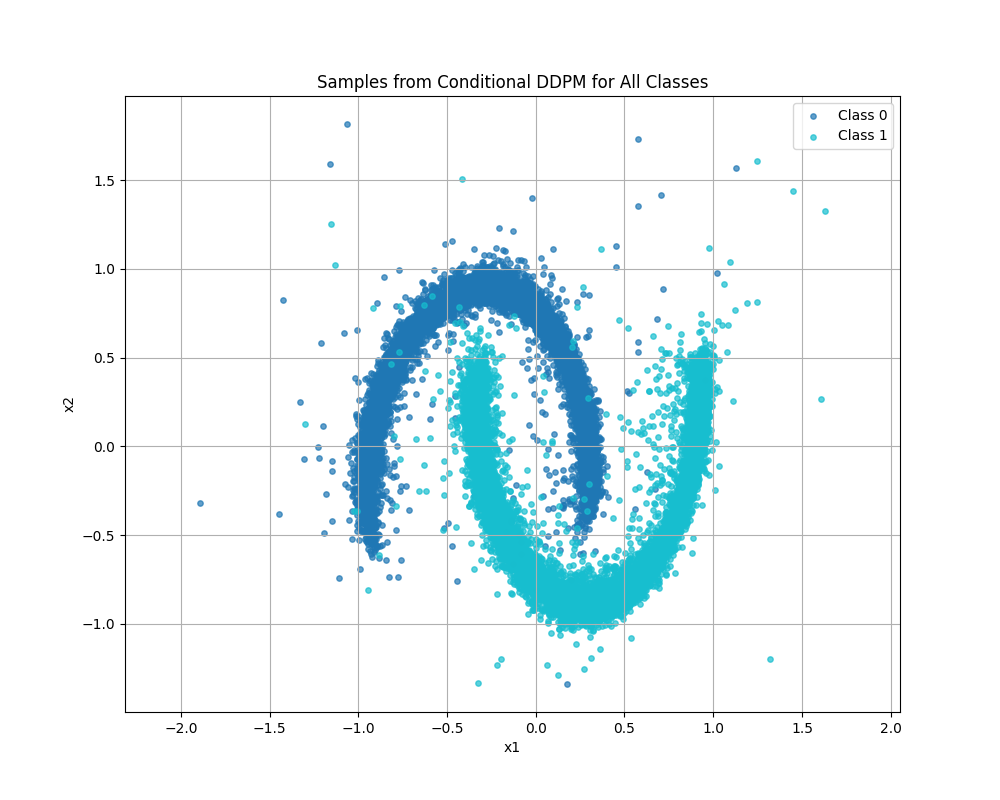
\includegraphics[width=\linewidth]{"images/Samples - CFG for cond_ddpm_2_50_0.0001_0.02_moons_0.0_sigmoid.png"}
      \subcaption{Guidance Scale = 0 (Equivalent to Conditional Sampling)}
  \end{minipage}
  \begin{minipage}{0.3\textwidth}
      \centering
      \includegraphics[width=\linewidth]{"images/Samples - CFG for cond_ddpm_2_50_0.0001_0.02_moons_0.2_sigmoid.png"}
      \subcaption{Guidance Scale = 0.2}
  \end{minipage}

  \vspace{0.5cm}

  \begin{minipage}{0.3\textwidth}
      \centering
      \includegraphics[width=\linewidth]{"images/Samples - CFG for cond_ddpm_2_50_0.0001_0.02_moons_0.5_sigmoid.png"}
      \subcaption{Guidance Scale = 0.5}
  \end{minipage}
  \begin{minipage}{0.3\textwidth}
      \centering
      \includegraphics[width=\linewidth]{"images/Samples - CFG for cond_ddpm_2_50_0.0001_0.02_moons_0.7_sigmoid.png"}
      \subcaption{Guidance Scale = 0.7}
  \end{minipage}
  \begin{minipage}{0.3\textwidth}
      \centering
      \includegraphics[width=\linewidth]{"images/Samples - CFG for cond_ddpm_2_50_0.0001_0.02_moons_1.0_sigmoid.png"}
    \subcaption{Guidance Scale = 1.0}
  \end{minipage}

  \vspace{0.5cm}

  \begin{minipage}{0.3\textwidth}
      \centering
      \includegraphics[width=\linewidth]{"images/Samples - CFG for cond_ddpm_2_50_0.0001_0.02_moons_2.0_sigmoid.png"}
      \subcaption{Guidance Scale = 2.0}
  \end{minipage}
  \begin{minipage}{0.3\textwidth}
      \centering
      \includegraphics[width=\linewidth]{"images/Samples - CFG for cond_ddpm_2_50_0.0001_0.02_moons_4.0_sigmoid.png"}
      \subcaption{Guidance Scale = 4.0}
  \end{minipage}

  \caption{Moons - CFG}
\end{figure}


Here are the NLL values for the two class labels:

\begin{table}[h]
  \centering
  \begin{tabular}{|c|c|c|}
      \hline
      {\bf Guidance Scale} & {\bf NLL for Class Label 0} & {\bf NLL for Class Label 1} \\
      \hline
      0.0 & 0.53 & 0.58 \\
      0.2 & 0.51 & 0.58 \\
      0.5 & 0.50 & 0.59 \\
      0.7 & 0.50 & 0.60 \\
      1.0 & 0.51 & 0.62 \\
      2.0 & 0.57 & 0.66 \\
      4.0 & 0.65 & 0.71 \\
      \hline
  \end{tabular}
  \caption{NLL Values for the two class labels of the Moons Dataset}
  \label{tab:nll_values}
\end{table}


As, it is evident from the NLL values and the images shown above, guidance scales 0.2 and 0.5 perform the best. With higher guidance scales, we typically lose focus on randomly generated data, and rely too much on the training labels provided, thus the NLL values are low, when another sample is chosen from the actual dataset. These observations match with the ones presented in the CFG paper too.


We had also compared the samples generated with a simple classifier model trained, here are the accuracy results across various guidance scale values:



\begin{table}[h]
  \centering
  \begin{tabular}{|c|c|c|}
      \hline
      {\bf Guidance Scale} & {\bf Accuracy for Class Label 0} & {\bf Accuracy for Class Label 1} \\
      \hline
      0.0 & 0.52 & 0.49 \\
      0.2 & 0.52 & 0.50 \\
      0.5 & 0.52 & 0.51 \\
      0.7 & 0.52 & 0.52 \\
      1.0 & 0.52 & 0.52 \\
      2.0 & 0.49 & 0.55 \\
      4.0 & 0.46 & 0.61 \\
      8.0 & 0.44 & 0.67 \\
      10.0 & 0.44 & 0.68 \\
      \hline
  \end{tabular}
  \caption{Accuracy Values for the two class labels of the Moons Dataset}
  \label{tab:acc_values}
\end{table}


As we can see, the accuracy values do not vary much across various guidance scale values. They peak around a scale of 1 (which is as per the results obtained in the paper), similar to NLL results. Higher scale values tend to bias towards one of the class labels as demonstrated in the images too. 




\subsection*{Classifier using Conditional DDPM}

The \texttt{ClassifierDDPM} class implements a classification method using a Diffusion Probabilistic Model (DDPM). The classification is performed by computing the likelihood of each class given the input, using a pre-trained conditional DDPM.

Given an input $x \in \mathbb{R}^d$, we generate a noisy sample $x_t$ at a fixed timestep $t$ using the variance-preserving noise schedule:
\begin{equation}
x_t = \sqrt{\bar{\alpha}_t} x + \sqrt{1 - \bar{\alpha}_t} \epsilon,
\end{equation}
where:
\begin{itemize}
\item $\bar{\alpha}_t$ is the cumulative product of noise scheduling parameters,
\item $\epsilon \sim \mathcal{N}(0, I)$ is Gaussian noise.
\end{itemize}


For each class label $c \in {0, 1, \dots, C-1}$, the classifier uses the conditional DDPM model to predict the noise:
\begin{equation}
\hat{\epsilon}_c = \text{model}(x_t, t, c),
\end{equation}
where $\hat{\epsilon}_c$ is the predicted noise when conditioning on class $c$.

The classification score for class $c$ is computed as the negative mean squared error between the predicted and actual noise:
\begin{equation}
S_c = -\mathbb{E} \left[ | \hat{\epsilon}_c - \epsilon |^2 \right].
\end{equation}

This score measures how well the model’s noise prediction aligns with the actual noise for each class. A lower error implies a higher likelihood of the class being correct.

To convert the classification scores into probabilities, a softmax function is applied:
\begin{equation}
P(c \mid x) = \frac{\exp(S_c)}{\sum_{c'} \exp(S_{c'})}.
\end{equation}

The predicted class is then obtained as:
\begin{equation}
\hat{c} = \arg\max_c P(c \mid x).
\end{equation}

Let us now compare this classifier with the one trained for the previous part (we will calculate the accuracy of both of these classifiers from the data generated).

\begin{table}[h]
  \centering
  \begin{tabular}{|c|c|c|}
      \hline
      {\bf Dataset} & {\bf Trained Classifier Accuracy} & {\bf ClassifierDDPM Accuracy} \\
      \hline
      Moons & 100\% & 40.81\% \\
      Blobs & 96.88\% & 71.62\%\\
      Circles & 100.00 \% & 45.69\% \\
      Manycircles & 85.69\% & 13.31 \%\\
      \hline
  \end{tabular}
  \caption{Trained Classifier vs Classifier DDPM}
  \label{tab:classify}
\end{table}

As we can see, classifierDDPM performs quite badly as compared to the trained Classifier. It is quite low in case of manycircles, where the number of classes are large in number, as compared to other datasets.




\clearpage



\section*{Reward Guidance}

Denoising Diffusion Probabilistic Models (DDPM) generate samples by progressively denoising a noisy latent variable. The reverse process of diffusion is modeled using a conditional Gaussian distribution:

\begin{equation}
q(x_{t-1} | x_t) = \mathcal{N} (x_{t-1} ; \mu_t(x_t), \Sigma_t)
\end{equation}

where $\mu_t(x_t)$ is the \textbf{posterior mean estimate} at step $t$. In DDPM, this mean is typically approximated using a \textbf{pre-trained noise predictor} $\epsilon_\theta(x_t, t)$, which estimates the noise added at timestep $t$:

\begin{equation}
\mu_t(x_t) = \frac{1}{\sqrt{\alpha_t}} \left( x_t - \frac{\beta_t}{\sqrt{1 - \bar{\alpha}t}} \epsilon_\theta(x_t, t) \right)
\end{equation}

where:

$\alpha_t, \beta_t$ are diffusion process parameters,

Soft Value-Based Decoding (SVDD) modifies the denoising process by introducing a \textbf{reward function} $R(x_t)$, which biases the sampling towards high-reward samples. The key idea is to adjust the \textbf{posterior mean approximation} using a value-based gradient:

\begin{equation}
\tilde{\mu}t(x_t) = \mu_t(x_t) + \lambda R(x_t) \nabla{x_t} \log p(x_t)
\end{equation}

where:

$R(x_t)$ is the reward function (e.g., classifier-based reward),

$\lambda$ (reward scale) controls the influence of the reward function,

$\nabla_{x_t} \log p(x_t)$ is an estimate of the score function (guiding towards high-reward regions).

Effectively, SVDD \textbf{shifts the denoising trajectory} toward samples that maximize the reward while still following the probabilistic structure of DDPM.

In practice, $\nabla_{x_t} \log p(x_t)$ is difficult to compute directly. Instead, we approximate it using:

\textbf{Energy-Based Models (EBMs)}: Estimate the log-probability of samples using a learned energy function.

\textbf{Pre-trained Classifiers}: If a classifier is available, we use its log-probability gradient as an approximation.

SVDD modifies the posterior mean approximation in DDPM by incorporating \textbf{reward-based adjustments}. This allows guiding the generative process \textbf{without explicit conditioning}, making it useful for sampling high-reward samples in an \textbf{unconditional} model.





\end{document}
